\section{Ejercicio 1: Conexión a datos de Power BI - Tarea 4: Combinar datos} 

1. In File Explorer, browse to the D:/Labfiles/Lab06/Starter/Project folder, and then open the
States.xlsx file.\\

	\begin{center}
	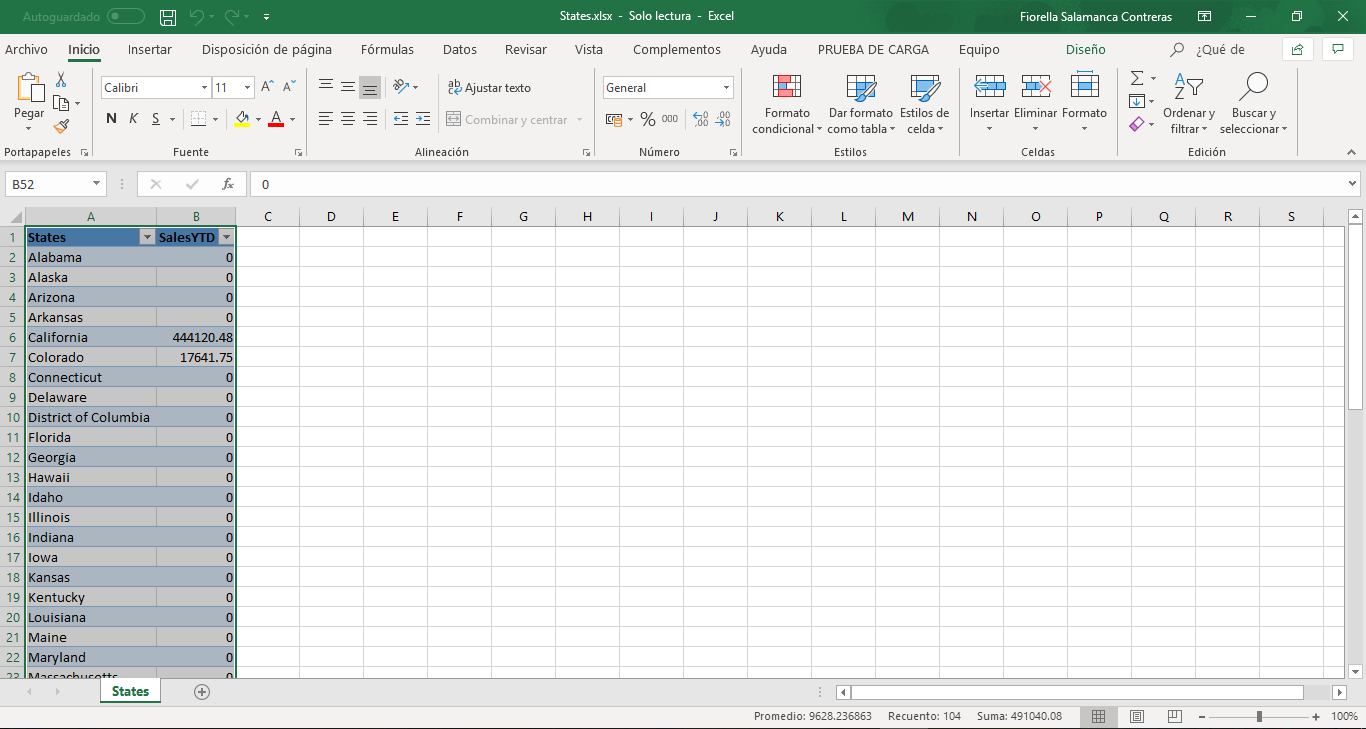
\includegraphics[width=17cm]{./Imagenes/Ejercicio1/Tarea4/1}
	\end{center}	

2. In the States worksheet, select all of the values in the two columns, and then press Ctrl+C.\\
3. In Power BI Desktop, on the Home ribbon, click Enter Data.\\

	\begin{center}
	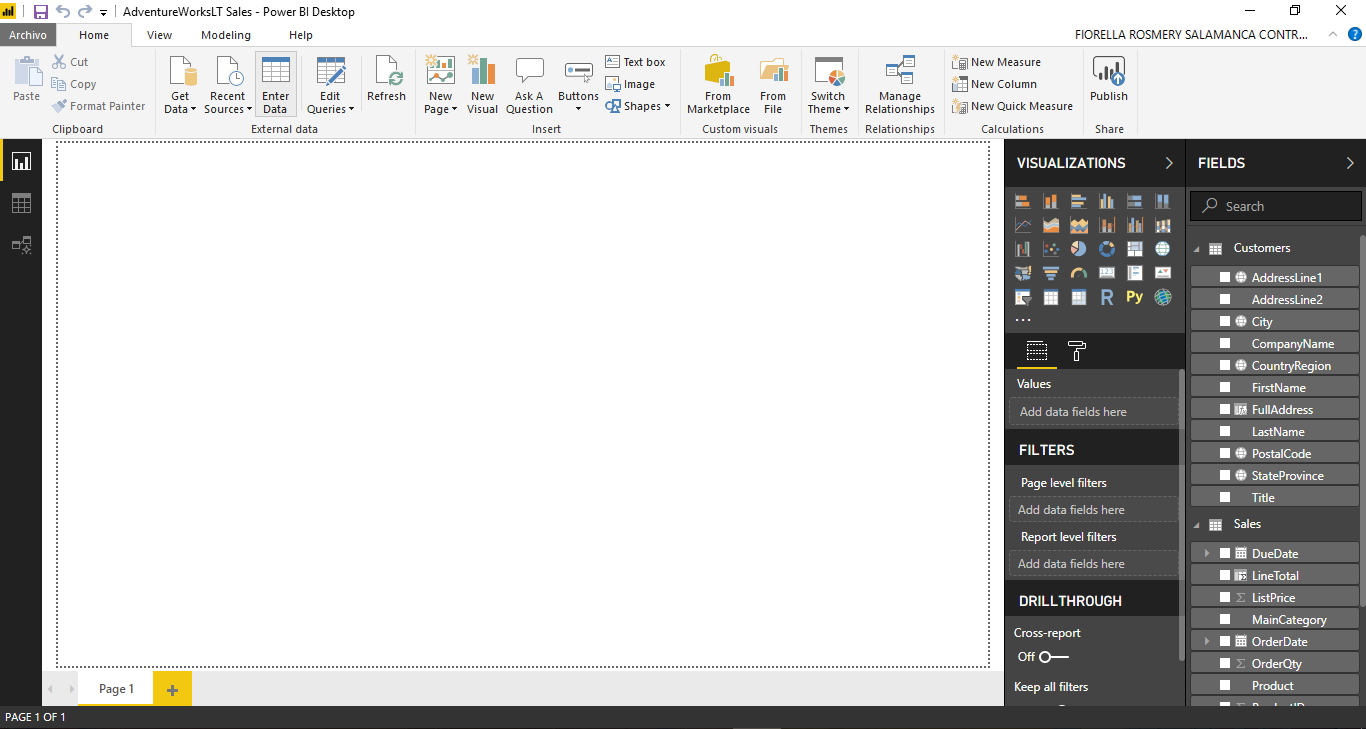
\includegraphics[width=17cm]{./Imagenes/Ejercicio1/Tarea4/2}
	\end{center}	

4. In the Create Table dialog box, click in the table, and then press Ctrl+V. Power BI detects that the first row is a column header.\\
5. In the Name box, type Sales by State, and then click Load.\\

	\begin{center}
	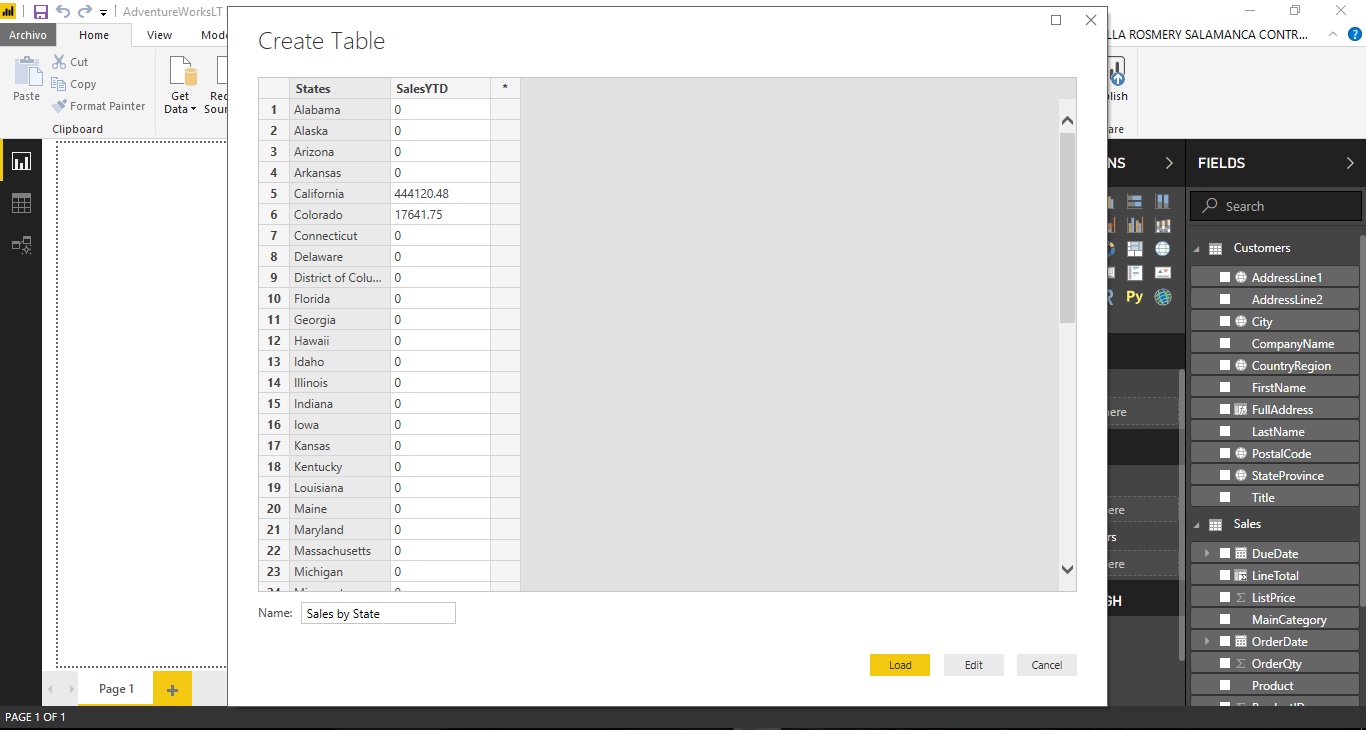
\includegraphics[width=17cm]{./Imagenes/Ejercicio1/Tarea4/3}
	\end{center}	

6. On the Home ribbon, click Get Data, and then click Web.\\

	\begin{center}
	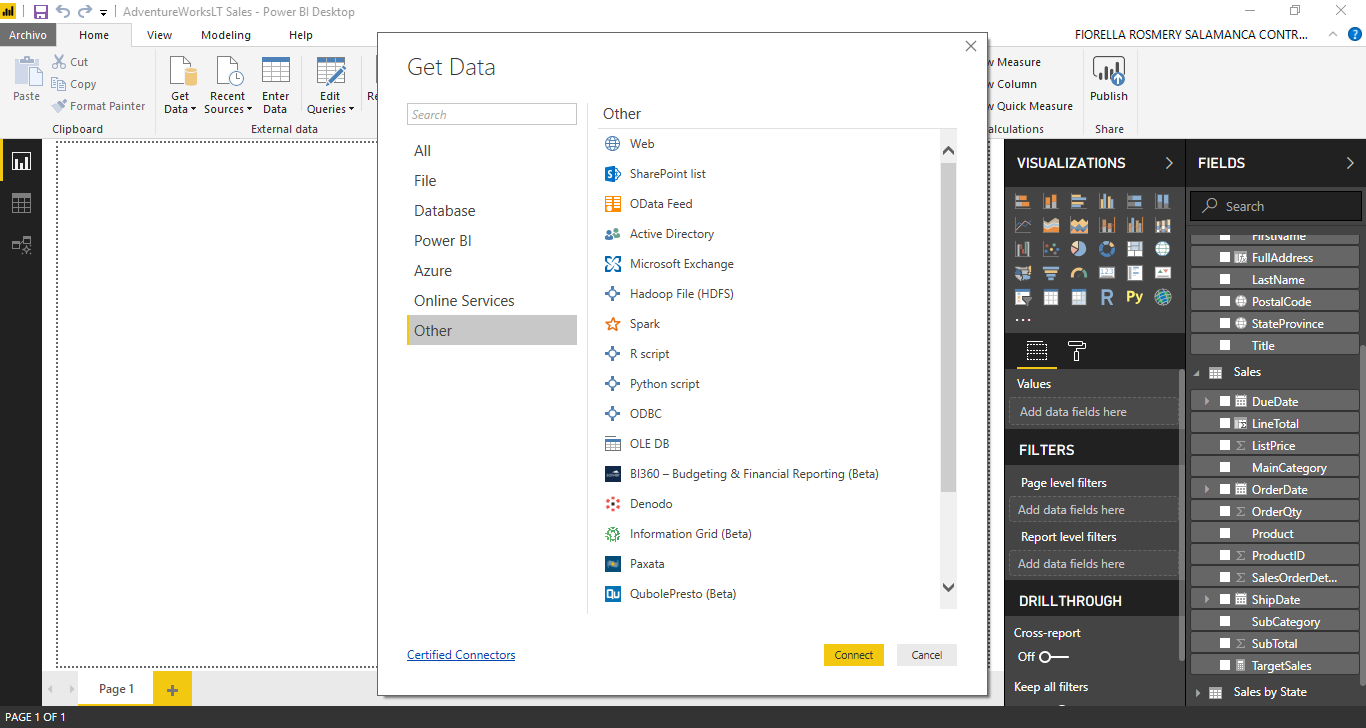
\includegraphics[width=17cm]{./Imagenes/Ejercicio1/Tarea4/4}
	\end{center}	


7. In the From Web dialog box, in the URL box, type http://en.wikipedia.org/wiki/List\_of\_U.S.\_state\_abbreviations, and then click OK.\\

	\begin{center}
	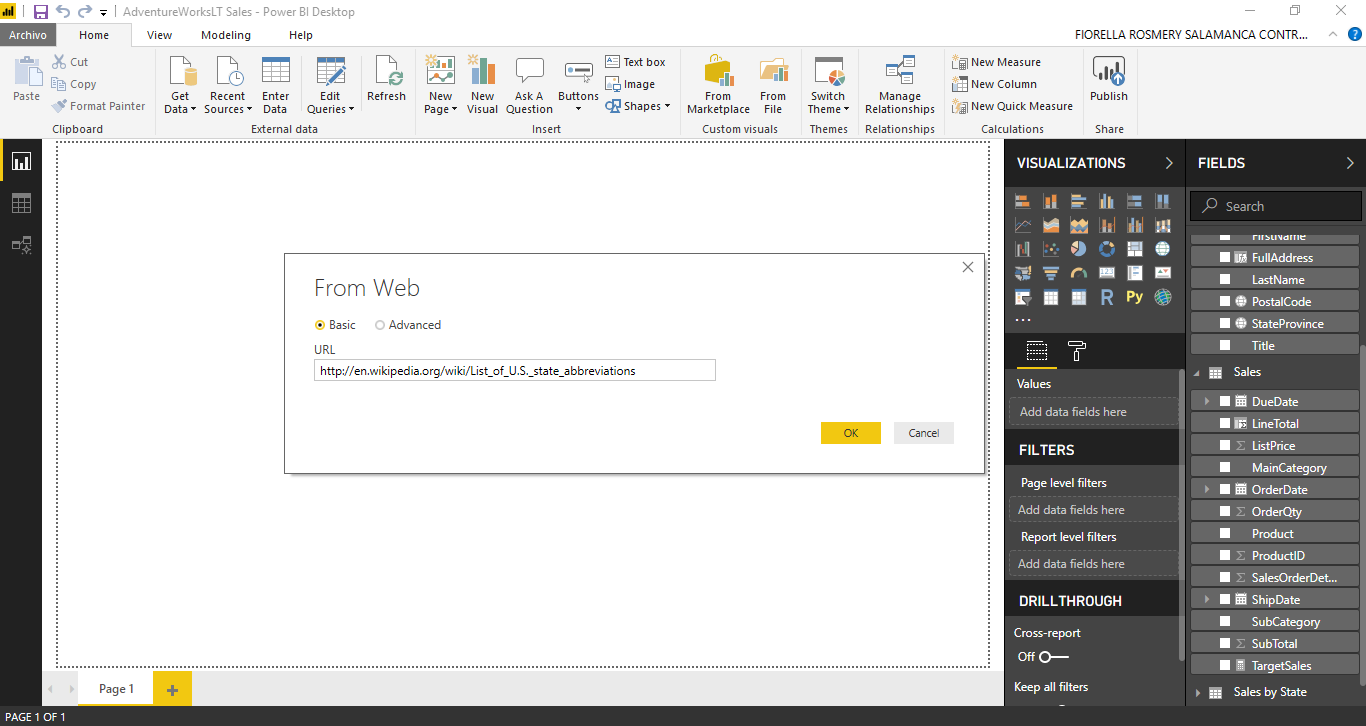
\includegraphics[width=17cm]{./Imagenes/Ejercicio1/Tarea4/5}
	\end{center}	

8. In the Navigator dialog box, select Codes and abbreviations for U.S. states, territories and other regions, and then click Load.\\

	\begin{center}
	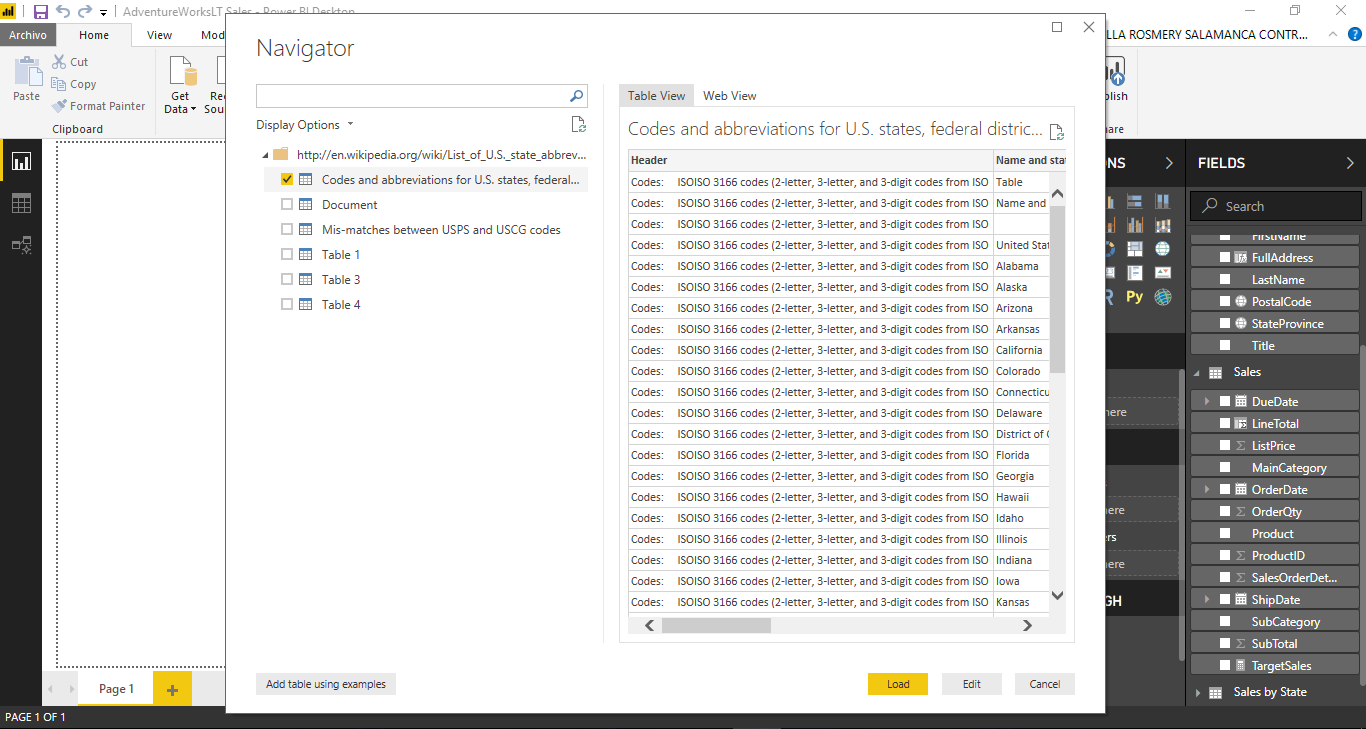
\includegraphics[width=17cm]{./Imagenes/Ejercicio1/Tarea4/6}
	\end{center}	

9. In the Fields pane, click Codes and abbreviations for U.S. states, territories and other regions to display the data. The table has 26 rows at the bottom that are not needed.\\

	\begin{center}
	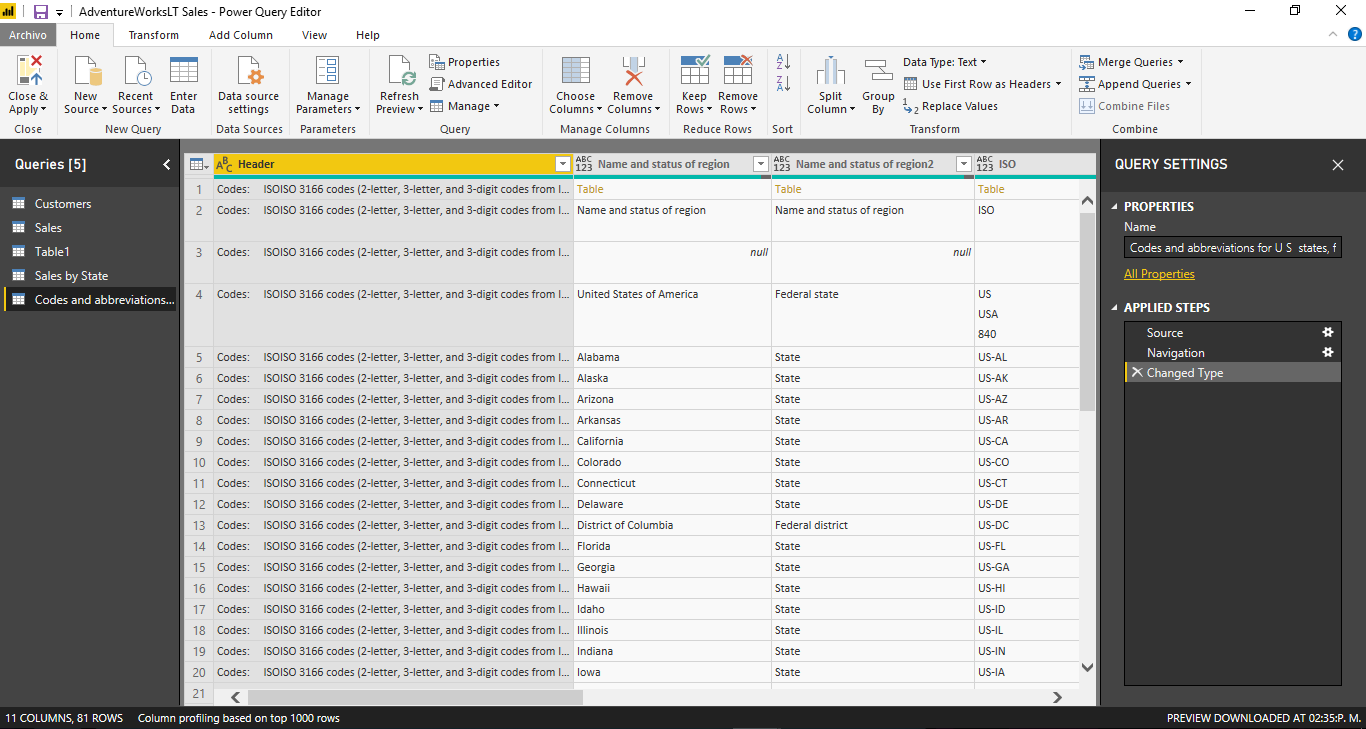
\includegraphics[width=17cm]{./Imagenes/Ejercicio1/Tarea4/7}
	\end{center}	

10. On the Home ribbon, in the External Data group, click Edit Queries, then click Edit Queries.\\
11. In Query Editor, in the Queries pane, click Codes and abbreviations for U.S. states, territories and
other regions.\\
12. On the Home ribbon, click Reduce Rows, click Remove Rows, and then click Remove Bottom
Rows.\\

	\begin{center}
	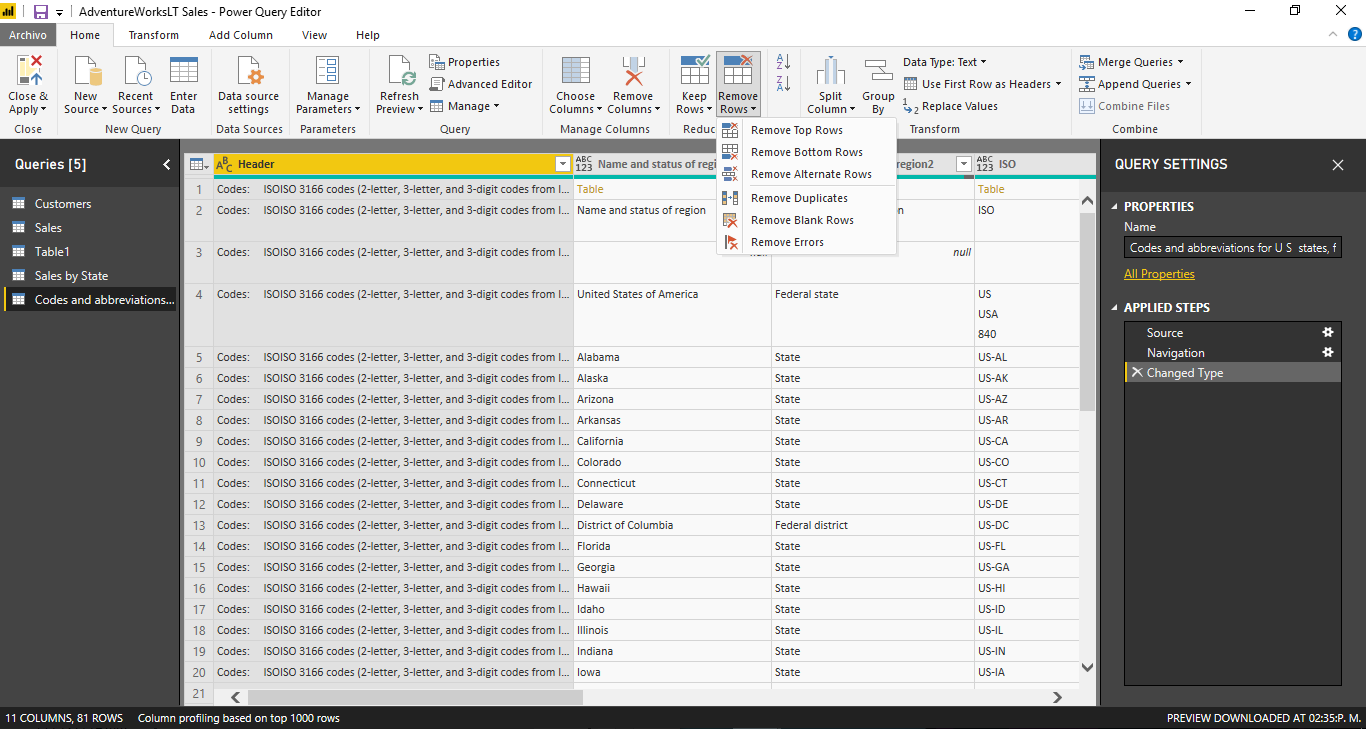
\includegraphics[width=17cm]{./Imagenes/Ejercicio1/Tarea4/8}
	\end{center}	

13. In the Remove Bottom Rows dialog box, in the Number of rows box, type 26, and then click OK.\\

	\begin{center}
	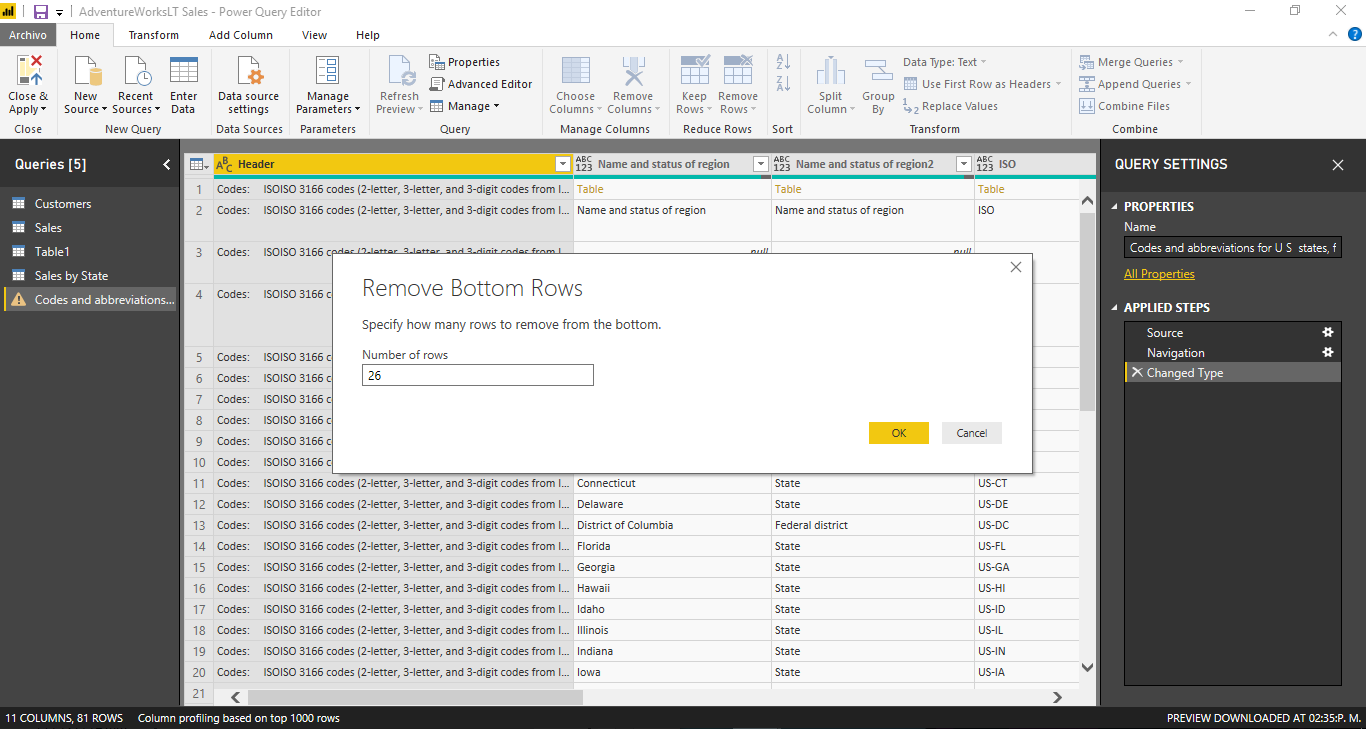
\includegraphics[width=17cm]{./Imagenes/Ejercicio1/Tarea4/9}
	\end{center}	

14. Click the ANSI2 column header, and then hold down the Ctrl key while selecting all of the columns to
the right. This selects multiple rows.\\

	\begin{center}
	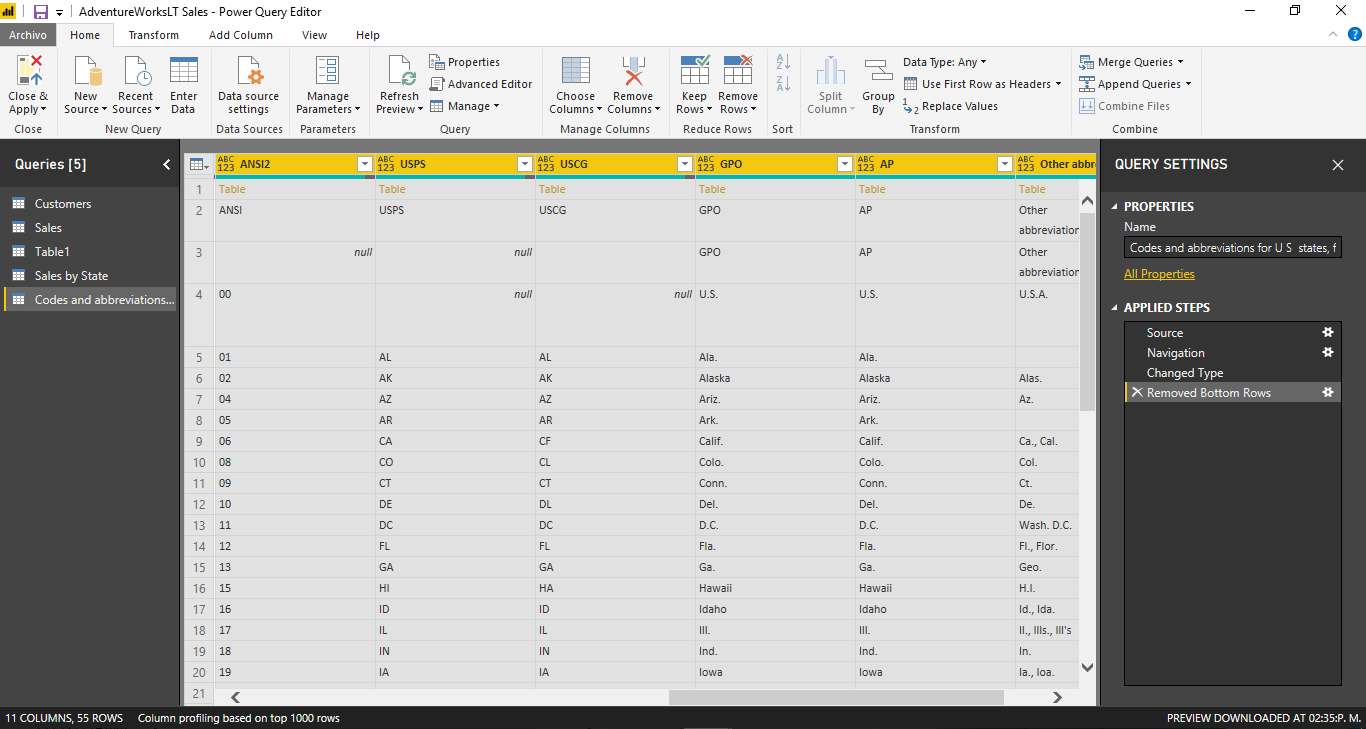
\includegraphics[width=17cm]{./Imagenes/Ejercicio1/Tarea4/10}
	\end{center}	

15. Still holding down Ctrl, click the Name and status of region2 and Header columns to include this in
the selection.\\

	\begin{center}
	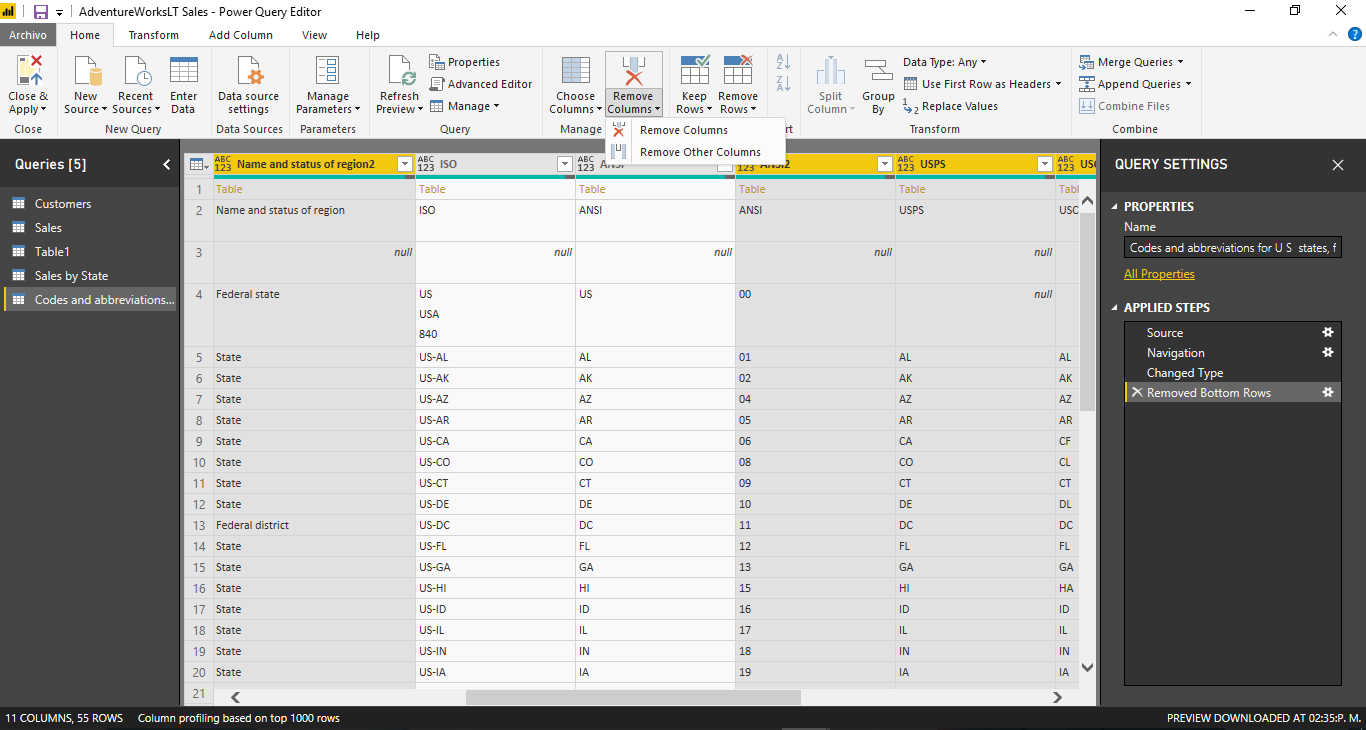
\includegraphics[width=17cm]{./Imagenes/Ejercicio1/Tarea4/11}
	\end{center}	

16. On the Home ribbon, click Manage Columns, click Remove Columns, and then click Remove Columns.\\
17. In the Query Settings pane, under Properties, in the Name box, type States with Codes, and then
press Enter.\\

	\begin{center}
	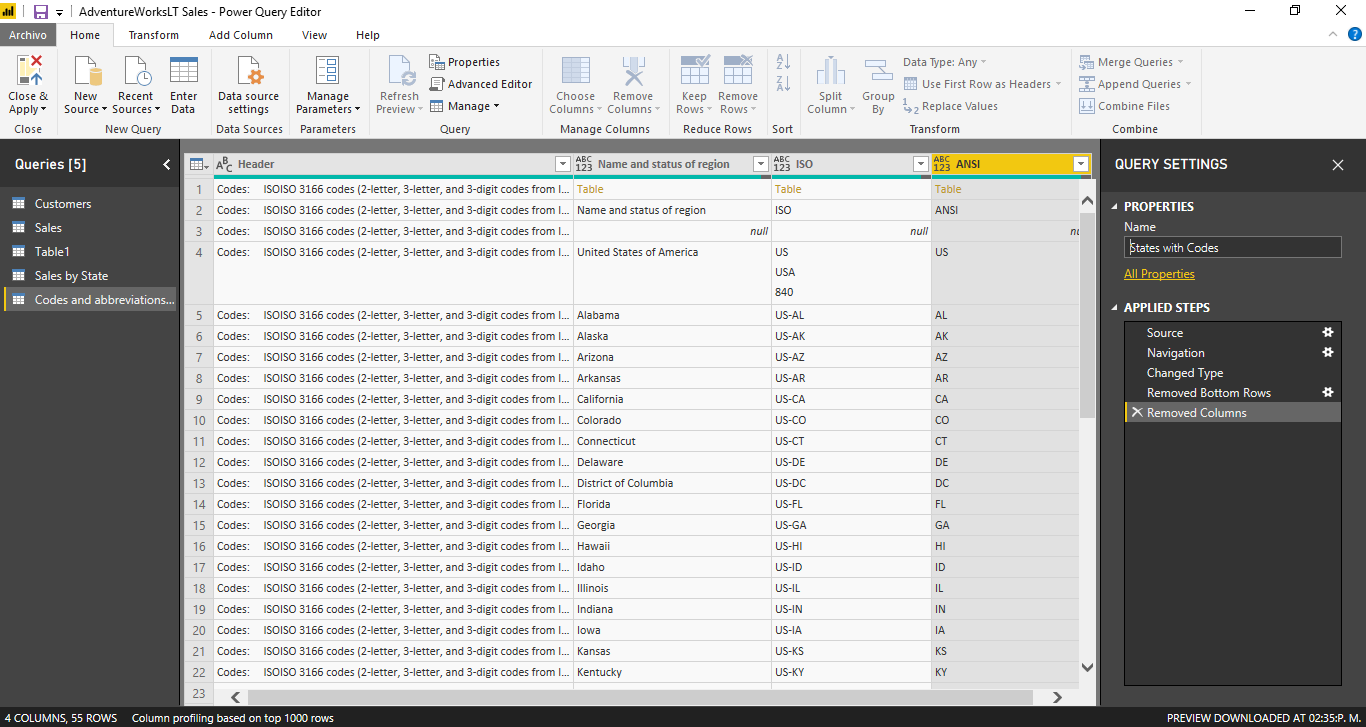
\includegraphics[width=17cm]{./Imagenes/Ejercicio1/Tarea4/12}
	\end{center}	

18. On the Home ribbon, in the Transform group, click Use First Row as Headers.\\
19. Right-click the United States of America column header, click Rename, type State Name, and then
press Enter.\\

	\begin{center}
	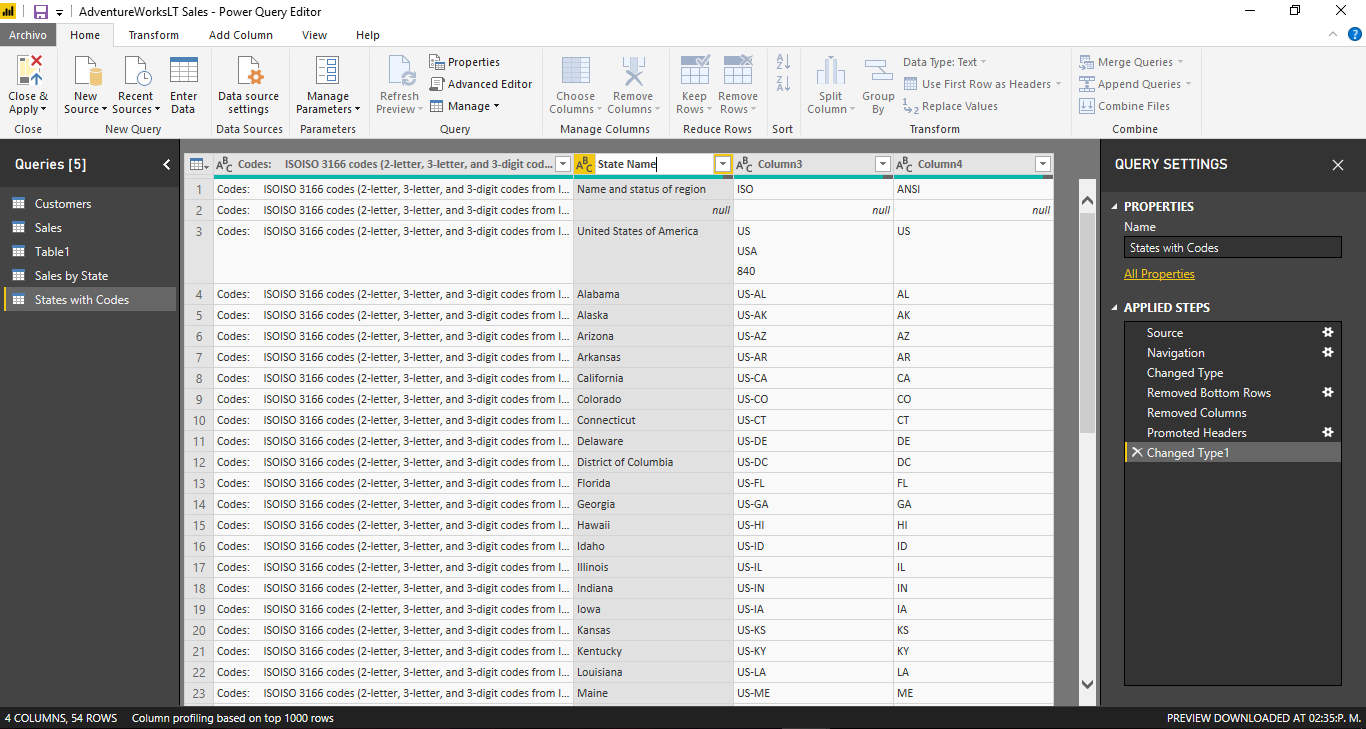
\includegraphics[width=17cm]{./Imagenes/Ejercicio1/Tarea4/13}
	\end{center}	

20. Right-click the US USA 840 column header, click Rename, type State Code Long, and then press
Enter.\\

	\begin{center}
	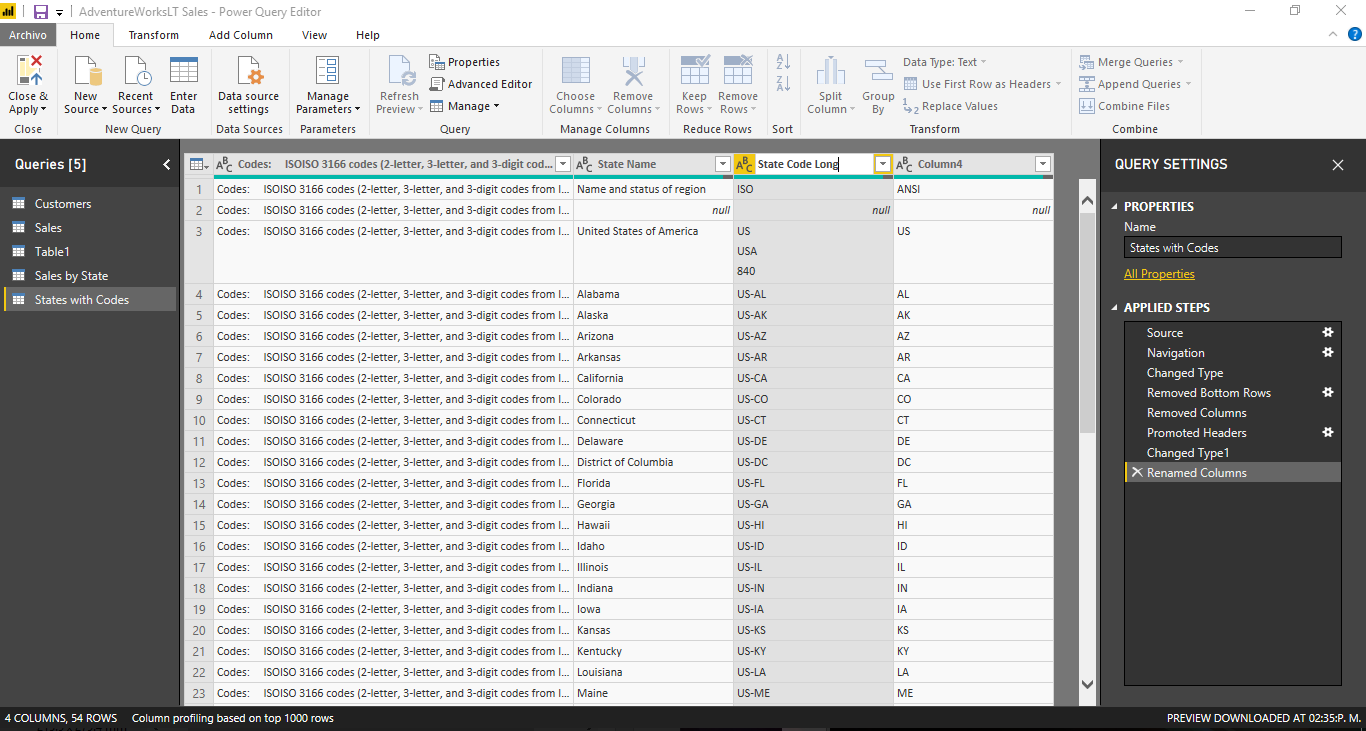
\includegraphics[width=17cm]{./Imagenes/Ejercicio1/Tarea4/14}
	\end{center}	

21. Right-click the US column header, click Rename, type State Code Short, and then press Enter.\\

	\begin{center}
	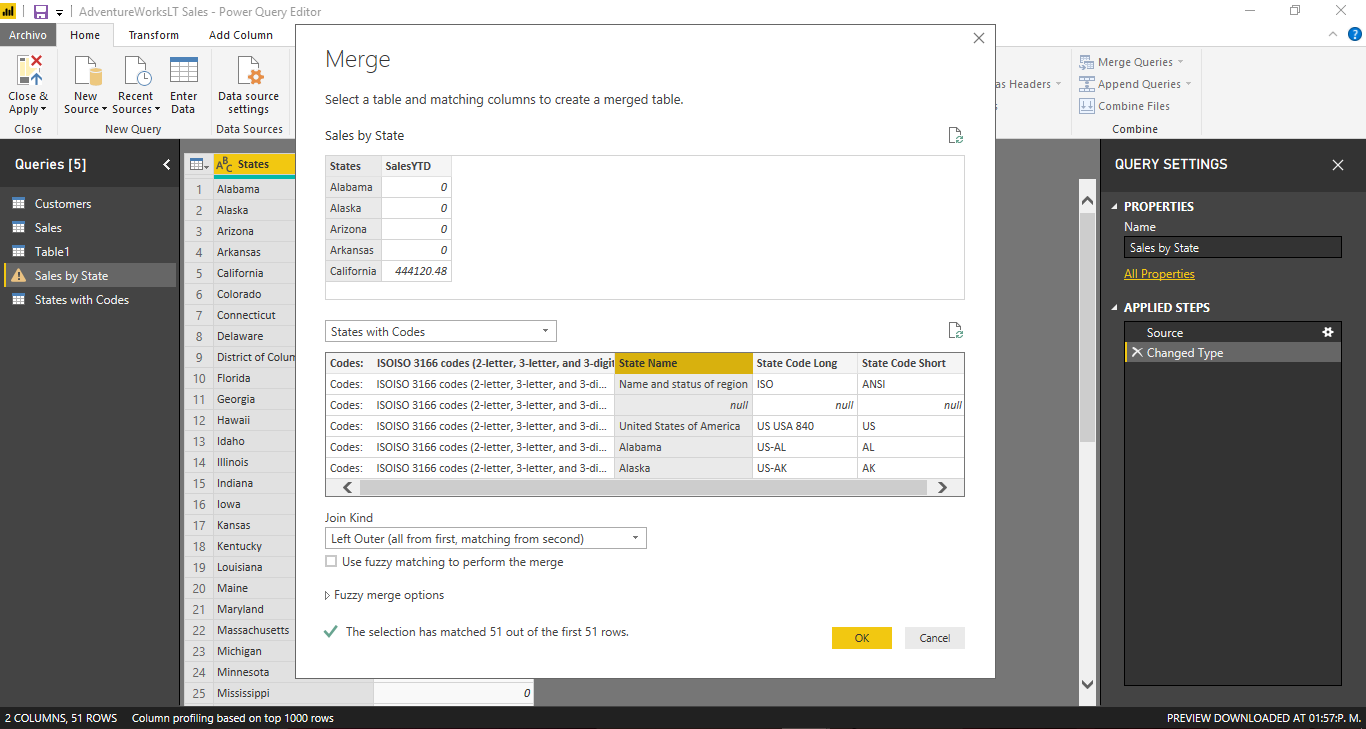
\includegraphics[width=17cm]{./Imagenes/Ejercicio1/Tarea4/16}
	\end{center}	

22. In the Queries pane, click Sales by State.\\
23. On the Home ribbon, click Combine, and then click Merge Queries.\\
24. In the Merge dialog box, in the Sales by State table, click the States column.\\
25. In the list, click States with Codes, click the State Name column, and then click OK. The new column
is added to the table and contains the merged States with Codes table.\\

	\begin{center}
	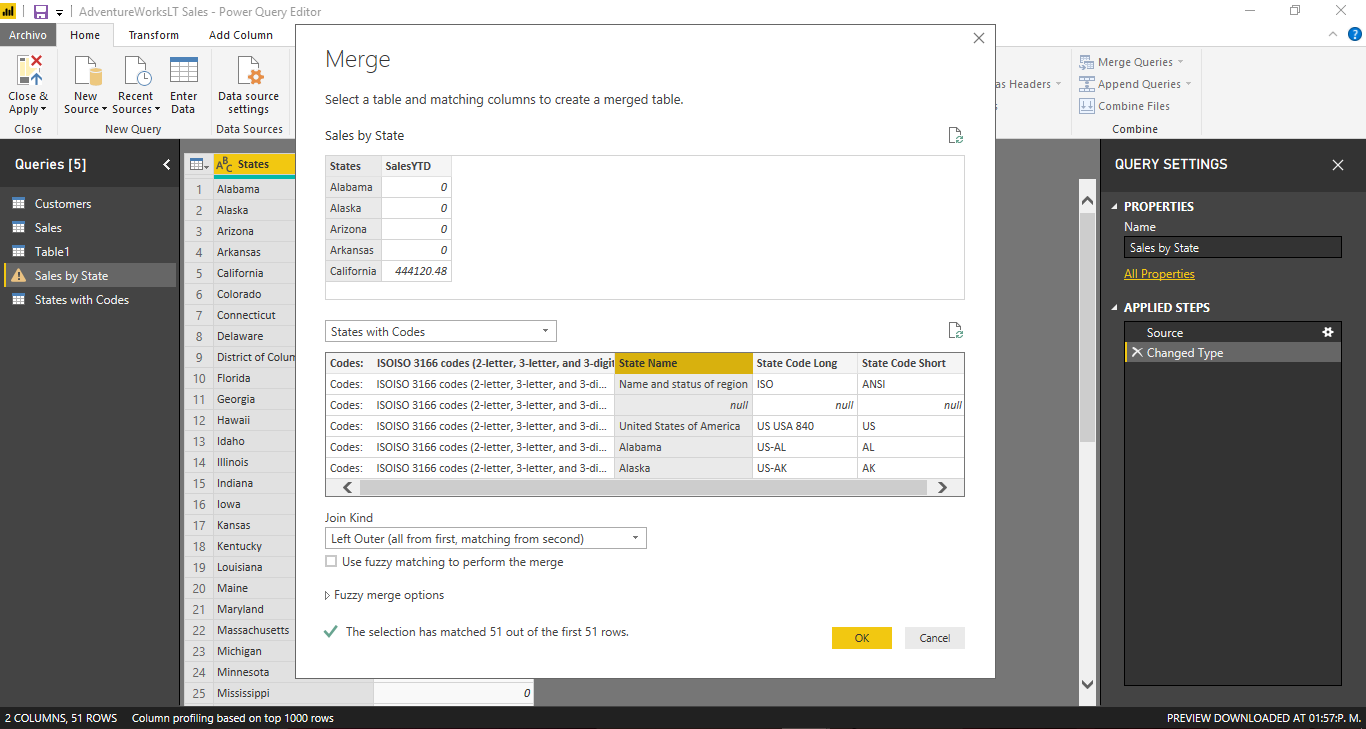
\includegraphics[width=17cm]{./Imagenes/Ejercicio1/Tarea4/16}
	\end{center}	

26. In the column header, click the Expand icon, clear (Select All Columns), select State Code Short,
and then click OK. The column now shows just the state codes.\\

	\begin{center}
	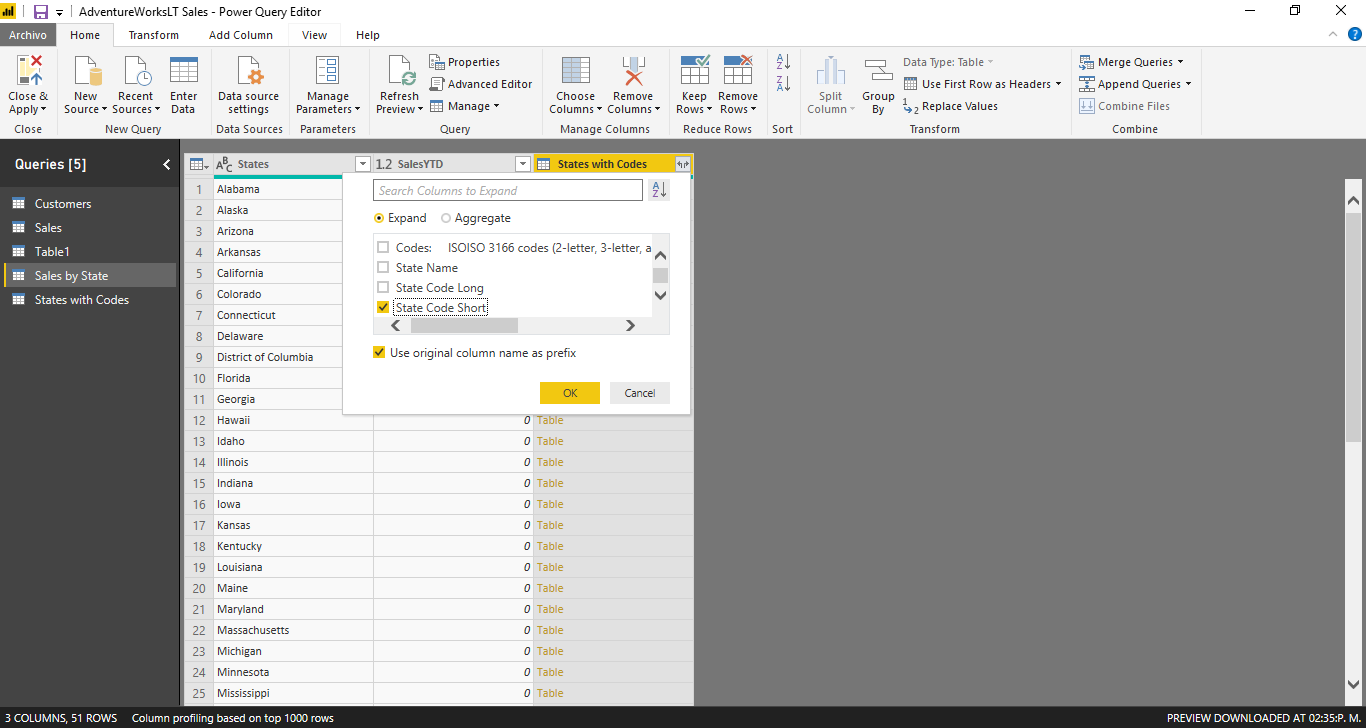
\includegraphics[width=17cm]{./Imagenes/Ejercicio1/Tarea4/17}
	\end{center}	

27. Right-click the column, click Rename, type State Code, and then press Enter.\\
28. On the File menu, click Close \& Apply.\\

	\begin{center}
	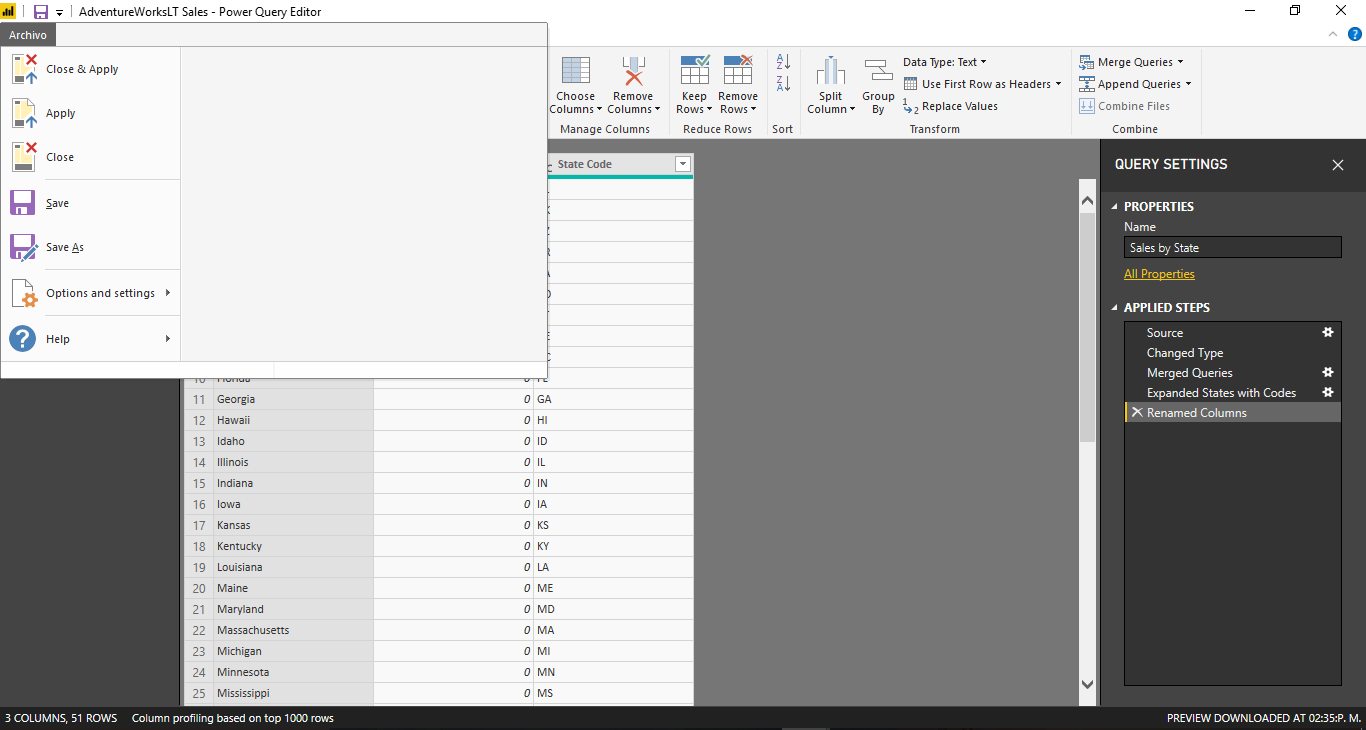
\includegraphics[width=17cm]{./Imagenes/Ejercicio1/Tarea4/18}
	\end{center}	

29. In the Fields pane, right-click States with Codes, and then click Hide in Report View.\\

	\begin{center}
	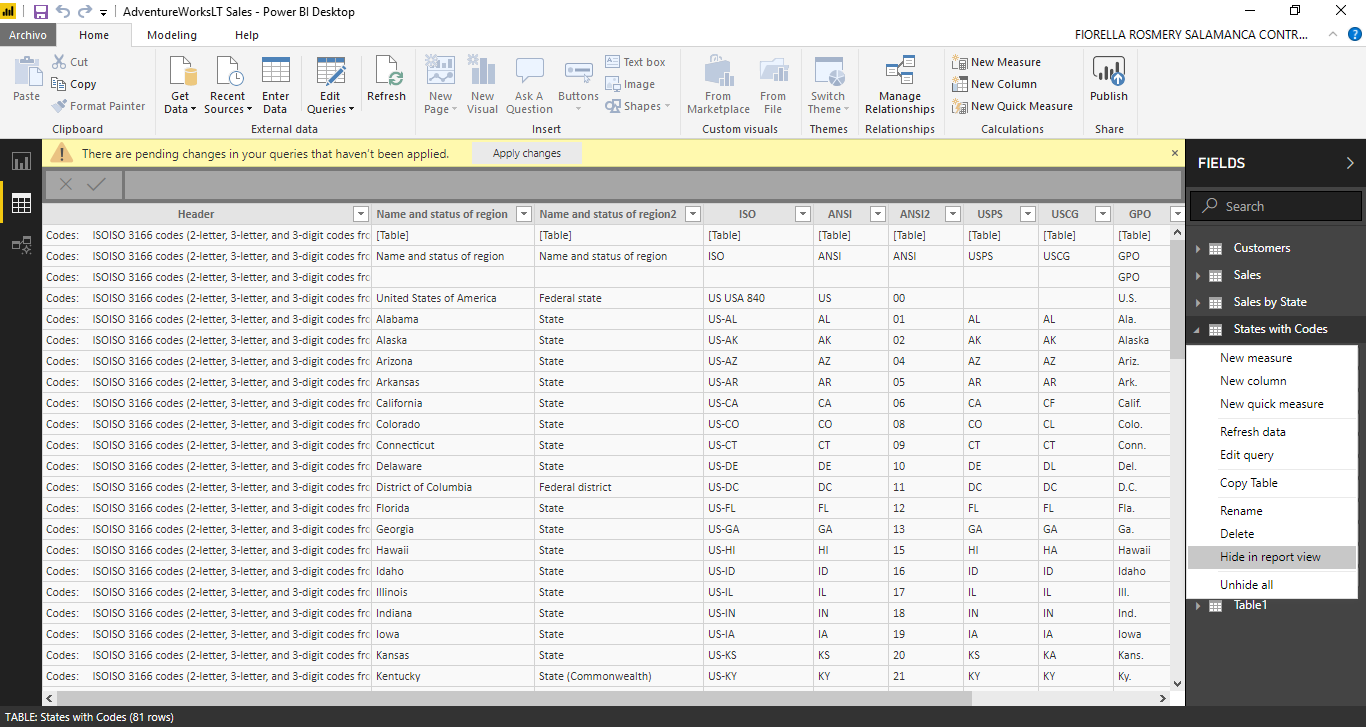
\includegraphics[width=17cm]{./Imagenes/Ejercicio1/Tarea4/19}
	\end{center}	

Results: After this exercise, you should have imported data from Azure, shaped it by using the Power BI
transformation tools, and combined the data by merging columns and appending rows.\\